% !TEX root = ./main.tex
% !TEX encoding = UTF-8 Unicode
% !TEX program = pdflatex
% !TeX spellcheck = it_IT

\chapter{Caricamento dati}
In questo capitolo verrono mostrate le operazioni effettuare per il caricamento
dei dati in MongoDB e per il collegamento di Databricks a MongoDB.

\section{Caricamento dati in MongoDB}
Come già detto in precedenza MongoDB è stato installato su di un singolo nodo.
Dopo averlo installa è stato lanciato il servizio \textbf{\textit{mongod}} è stato
possibile laciare da remoto il comando per l'import dei dati in formato JSON.
Di seguito è riportato uno degli importo effettuati.

\begin{figure}[!htbp]
	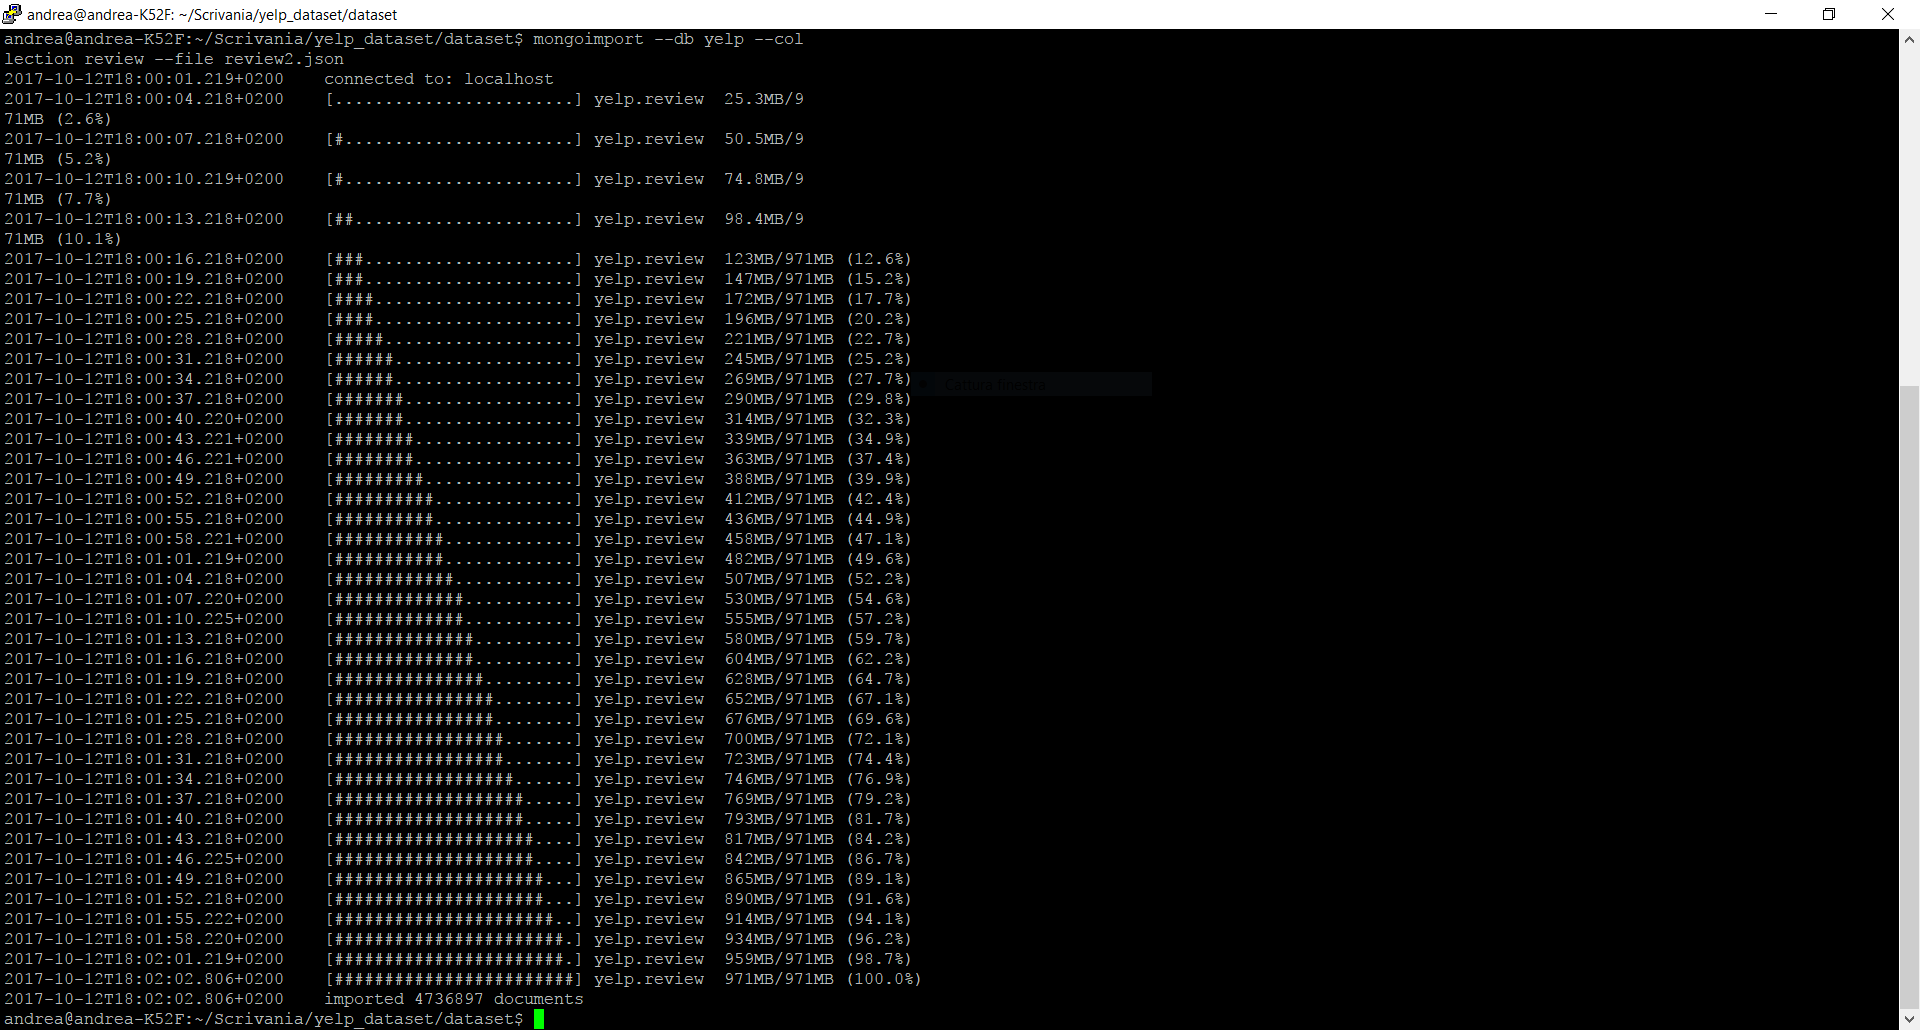
\includegraphics[width=.7\linewidth,keepaspectratio]{load_on_mongo}
  \caption{Apache Spark}
  \label{}
\end{figure}


\section{Da MongoDB a Databricks}

Per la connessione di MongoDB a Databricks è stato necessario scaricare il connettore
da caricare nella piattaforma di destinazione. Di seguito è riportato il codice
scala necessario per l'import dei dati.

%% un immagine
